%%%%%%%%%%%%%%%%%%%%%%%%%%%%%%%%%%%%%%%%%%%%%%%%%%%%%%%%%%%%%%%%%%%%%%%%
% Plantilla TFG/TFM
% Escuela Politécnica Superior de la Universidad de Alicante
% Realizado por: Jose Manuel Requena Plens
% Contacto: info@jmrplens.com / Telegram:@jmrplens
%%%%%%%%%%%%%%%%%%%%%%%%%%%%%%%%%%%%%%%%%%%%%%%%%%%%%%%%%%%%%%%%%%%%%%%%

\chapter{Metodología}
\label{metodologia}

El desarrollo de este proyecto respeta tanto el proceso de desarrollo \textit{Software} como el ciclo de vida de proyectos de \textit{Ciencia de Datos}, por lo que se ha dividido en varias fases acontecidas que definiremos a continuación en base a la planificación mediante un \textit{Diagrama de Gantt}:

Este diagrama proporciona una visión de las fases de un proyecto y su estimación temporal, figura \eqref{GranttImage}.

\begin{figure}[H]
    \centering
    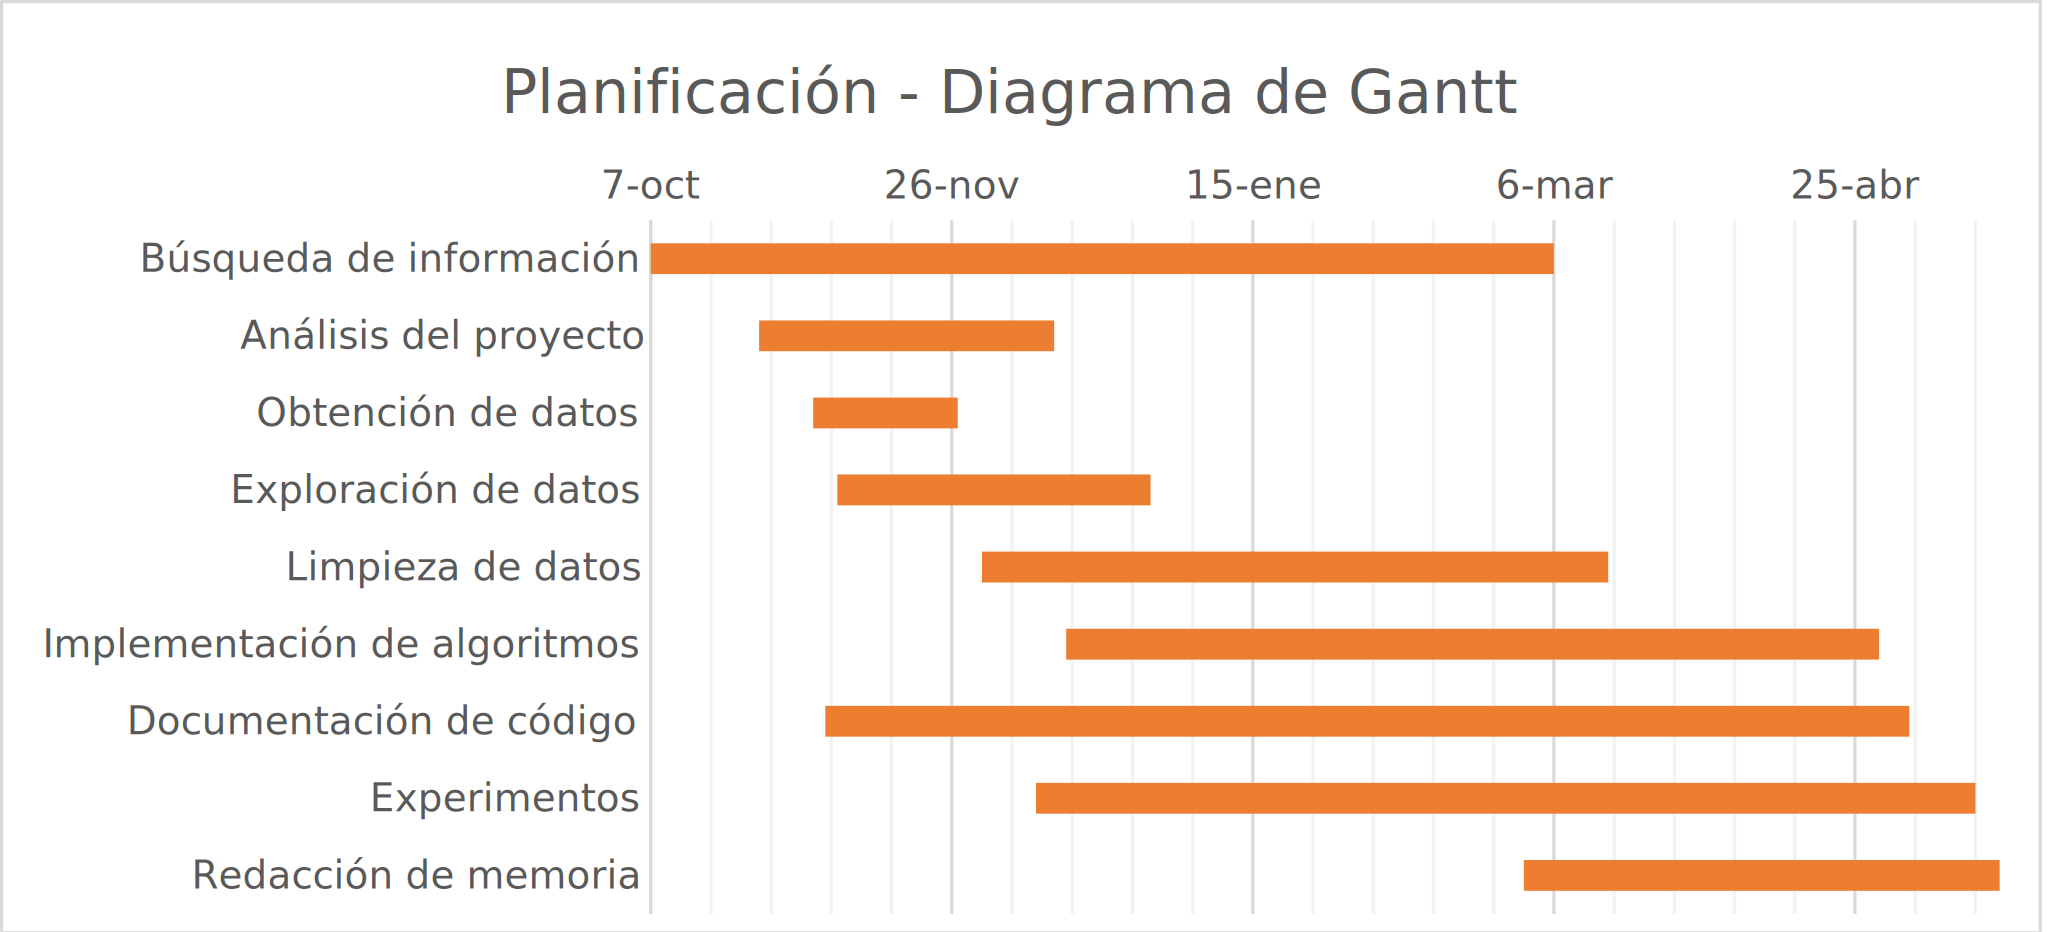
\includegraphics[width=15cm]{archivos/4.Metodologia/GranttImage}
    \caption{Diagrama de Gantt de la planificación del proyecto.}
    \label{GranttImage}
\end{figure}

La búsqueda de información incluye la investigación de todo lo referente al proyecto, y por este motivo, esta fase, es la primera en el desarrollo siendo un proceso que se ha prolongado durante casi toda la evolución del trabajo.

El análisis del proyecto consiste en estudiar la viabilidad del mismo, buscando fuentes de información desde las que poder obtener los datos además de explorarlos. Es una de las fases más críticas en un proyecto de \textit{Ciencia de Datos}, ya que si las conclusiones del estudio de viabilidad no son sólidas, se podría cometer el riesgo de empezar un proyecto en el que no es factible cubrir los objetivos.

La obtención de datos consiste en la búsqueda de repositorios donde encontrar datos que contengan la información requerida para abarcar los objetivos del proyecto. Se ha realizado visitando distintos portales de datos abiertos nacionales hasta encontrar un conjunto de datos que encajase con los objetivos, en esta fase también se involucra la exploración inicial de los datos.

La exploración de datos abarca la fase de análisis de datos, esto se realiza utilizando métodos visuales para entender las características propias del dataset, además de hacer una valoración de la calidad de los mismos. Las primeras etapas de esta fase se complementan con el análisis del proyecto.

El siguiente paso ha sido la limpieza de datos. Gracias a la exploración, se comprenden la naturaleza de los datos y se decide qué tecnicas usar para el tratamiento de valores atípicos del conjunto de datos para su posterior transfomación.

Una de las tareas más importantes en el ciclo de vida de desarrollo software, que garantizan la calidad del producto, es la documentación de código. Tiene como fin
clarificar conceptos y explicar el funcionamiento de los métodos que componen el desarrollo. Es una fase que se prolonga desde el inicio de la codificación en la limpieza de datos hasta poco tiempo después de terminar de implementar los modelos.

A nivel funcional, la última fase de este proyecto ha sido la realización de experimentos. Comienza poco antes que la implementación de los modelos y consiste en testar las distintas implementaciones, tanto de limpieza de datos como el funcionamiento de los modelos.

Finalmente hay que redactar la memoria, plasmando toda la información obtenida durante la evolución del proyecto.


\clearpage

\section{Fases}

    En esta sección describiremos cada uno de los pasos que ha seguido el desarrollo del proyecto, desde la búsqueda inicial de datos hasta la implementación final de los algoritmos. Para ello, un aspecto muy importante en un TFM es el diagrama de flujo de la metodología. En este diagrama se define el flujo de ejecución del proyecto y, como se puede observar en la figura \eqref{DataflowImage}, se han dividido las etapas del proyecto en seis bloques claramente diferenciados. Cada uno de estos está orientado a una disciplina distinta en proyectos de \textit{Ciencia de Datos} y por lo tanto serán detallados en cada una de las subsecciones posteriores.\\


    \begin{figure}[H]
        \centering
        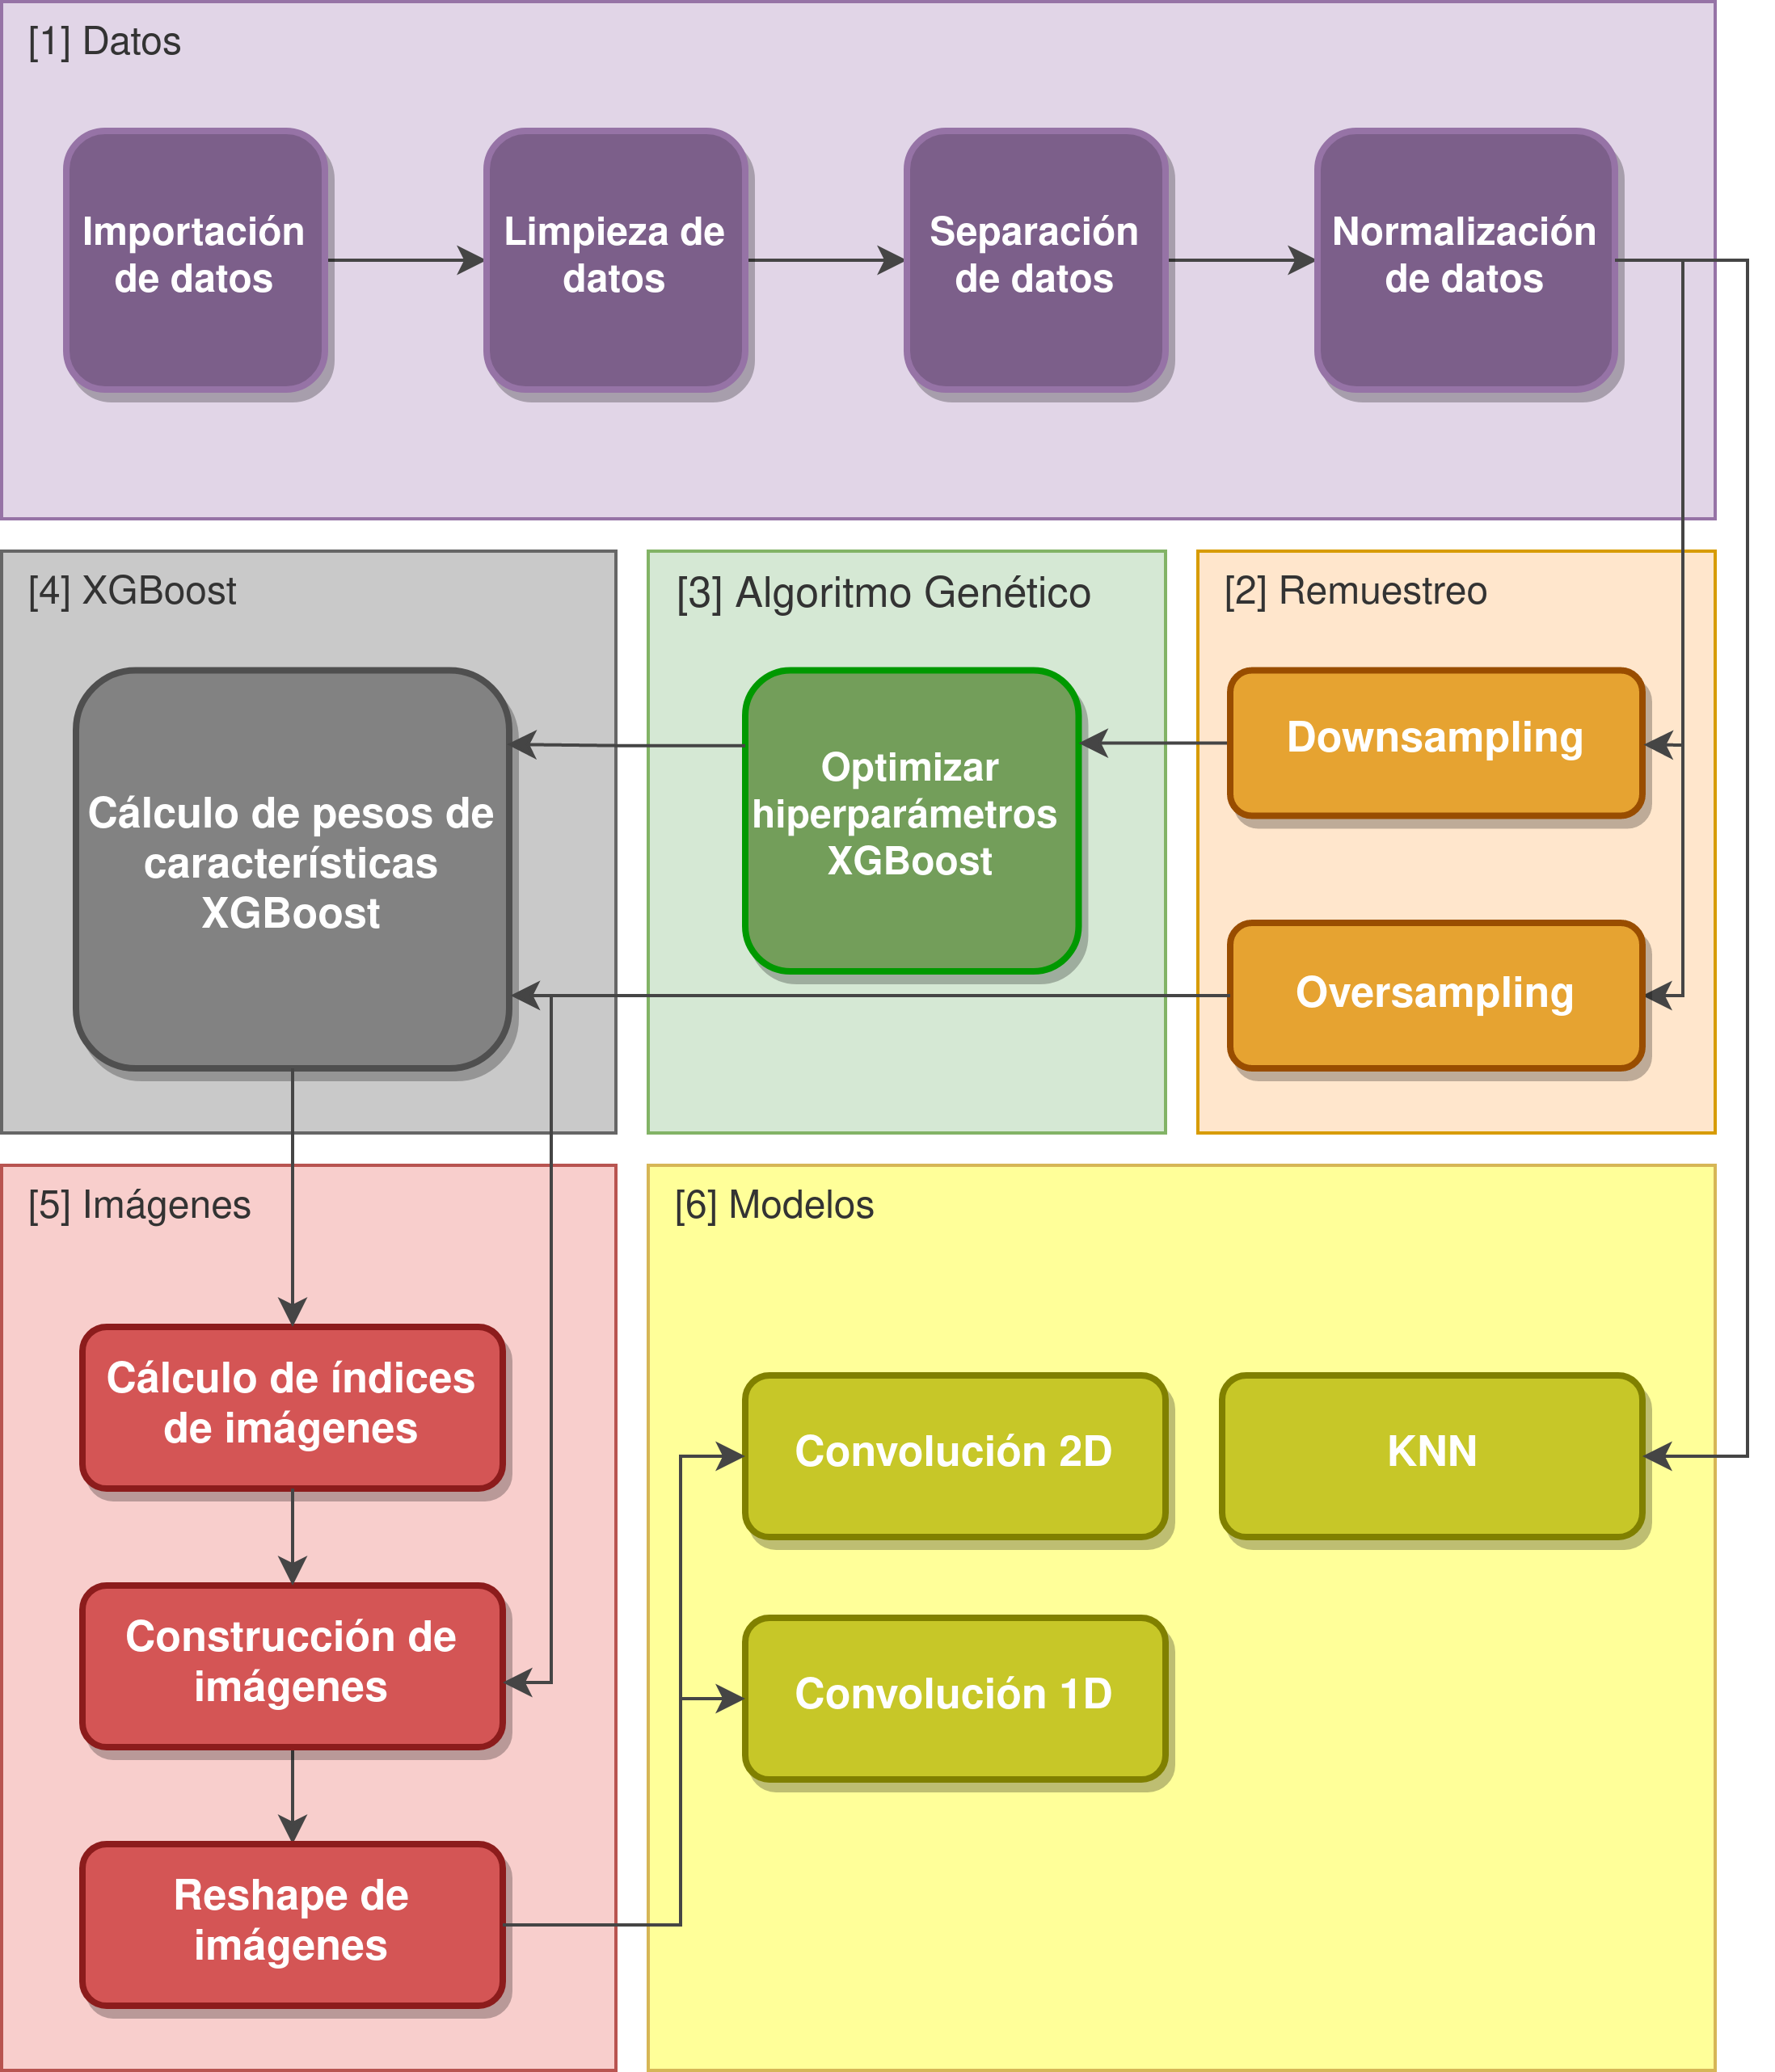
\includegraphics[width=13cm]{archivos/4.Metodologia/DataflowImageESP}
        \caption{Flujo de datos del proceso del proyecto.}
        \label{DataflowImage}
    \end{figure}



    \subsection{Datos}


            Como en cualquier proyecto de \textit{Ciencia de Datos} el primer paso contempla la obtención, preparación y estudio de los datos. Este es el proceso en el que más tiempo se invierte en el ciclo de vida de un proyecto, algunos estudios apuntan que alrededor del 80 por ciento del tiempo en un proyecto se destina a esta tarea \cite{LifecycleDataScienceProjectsTimes}, por lo que es extremadamente importante aplicar buenas prácticas a la hora de llevar a cabo esta fase.

            El conjunto de datos con el que se ha trabajado en este proyecto describe accidentes de tráfico de la ciudad de Madrid en un periodo concreto, desde el año 2019 hasta el 2022. Este dataset ha sido obtenido desde la web \cite{DatasetMadrid}, repositorio donde es posible encontrar distintos datasets relativos a la Comunidad de Madrid.

            El número total de registros en este periodo de tiempo es de 60.966 instancias, cada una de las cuales consta de 17 características que se describirán en la tabla \eqref{DescripcionDatosTabla}.

            \renewcommand{\arraystretch}{1.2}
            \begin{table}[h]
                \small
                \centering
                \begin{tabular}{|c|L{0.7\textwidth}|}
                    \hline
                    \textbf{Atributo}&\textbf{Descripción}\\
                    \hline
                    \texttt Número de expediente &
                    Identificador del incidente, si varios registros tienen el mismo número de expediente se consideran como un mismo accidente y cada registro representa cada una de las distintas personas involucradas en él (Conductor, Pasajero o Peatón).\\
                    
                    \hline
                    \texttt Fecha &
                    Día mes y año en el que se ha producido el incidente.\\
                    
                    \hline
                    \texttt Hora &
                    Hora y minuto del día.\\

                    \hline
                    \texttt Localización &
                    Nombre de la calle (si procede).\\

                    \hline
                    \texttt Número &
                    Número de la calle donde ha ocurrido el incidiente (si procede).\\

                    \hline
                    \texttt Distrito &
                    Nombre del distrito de Madrid donde ha ocurrido el incidente.\\

                    \hline
                    \texttt Tipo de accidente &
                    Tipología de accidente, puede ser de diversos tipos (Colisión doble, Colisión múltiple, Alcance, Choque contra obstáculo, Atropello, Vuelco, Caída, Otras causas).\\

                    \hline
                    \texttt Estado meteorológico &
                    Condiciones climatológicas en el momento del incidente (Despejado, Nublado, Lluvia débil, Lluvia intensa, Granizado o Nevando)\\

                    \hline
                    \texttt Tipo de vehículo &
                    Clasificación en función del tipo de vehículos, p.e. motocicleta, turismo, cuadriciclo, etc.\\

                    \hline
                    \texttt Tipo de persona &
                    Rol de la persona involucrada (Conductor, Pasajero o Peatón)\\

                    \hline
                    \texttt Rango de edad &
                    Intervalo de edad la persona implicada.\\

                    \hline
                    \texttt Sexo &
                    Sexo de la persona implicada (Hombre o Mujer).\\

                    \hline
                    \texttt Lesividad &
                    Consecuencias físicas de la persona implicada, si ha necesitado asistencia sanitaria, si ha sido ingresada o si ha sido mortal.\\

                    \hline
                    \texttt Coordenada X &
                    Coordenada X del accidente en formato \textit{UTM}.\\

                    \hline
                    \texttt Coordenada Y &
                    Coordenada Y del accidente en formato \textit{UTM}.\\

                    \hline
                    \texttt Positivo en alcohol &
                    Si la persona implicada ha dado positivo en el control de alcoholemia (S o N).\\

                    \hline
                    \texttt Positivo en drogas &
                    Si la persona implicada ha dado positivo en el control de estupefacientes (S o N).\\

                    \hline
                \end{tabular}
                \caption{Descripción de los datos.}
                \label{DescripcionDatosTabla}

            \end{table}


            Hay que resaltar la importancia del atributo lesividad, puesto que es la variable respuesta de este trabajo. Existen una serie de valores asignados a esta categoría, así cada dato de lesividad pertenece, al menos, a uno de los siguientes casos:

              \begin{itemize}
                    \item Consecuencias leves: comprende desde aquellas personas que no han resultado heridas hasta aquellas que han necesitado ingresar en un centro hospitalario no más de 24 horas. El tipado numérico de estas casuísticas es el siguiente:

                        \begin{itemize}
                            \item 1: Atención en urgencias sin posterior ingreso.
                            \item 2: Ingreso inferior o igual a 24 horas.
                            \item 5: Asistencia sanitaria ambulatoria con posterioridad.
                            \item 7: Asistencia sanitaria sólo en el lugar del accidente.
                            \item 14: Sin asistencia sanitaria.
                        \end{itemize}

                    \item Consecuencias severas: implicados que han requerido un ingreso hospitalario superior a 24 horas. En este caso el tipado numérico del conjunto de datos corresponde a:

                        \begin{itemize}
                            \item 3: Ingreso superior a 24 horas.
                        \end{itemize}

                    \item Consecuencias fatales: víctimas mortales dentro del margen de las 24 horas posteriores al accidente. La asignación numérica a este campo es:

                        \begin{itemize}
                            \item 4: Fallecido 24 horas.
                        \end{itemize}

                \end{itemize}


            Se pueden consultar más detalles de las características del dataset descripción del conjunto de datos del portal \textit{Open Data} de Madrid \cite{InfoDatasetMadrid}.


            \begin{enumerate}

                \item \textbf{Limpieza de datos}

                    Una vez importados los datos, es indisepensable hacer una limpieza de éstos, eligiendo las características que serán utilizadas como variables explicativas en las predicciones atendiendo además a los valores de las instancias, ya que pueden contener valores nulos, valores atípicos (\textit{outliers}) o contener valores erróneos. Esta problemática requiere de la aplicación de distintas fases de análisis.

                    En el caso del dataset de accidentes de tráfico de este proyecto se han escogido las siguientes características como variables explicativas: \textit{hora, distrito, tipo accidente, estado meteorológico, tipo vehiculo, tipo persona, rango edad, sexo, positivo alcohol, positivo drogas, vehiculos implicados, coordenada x utm, coordenada y utm}.


                    Una vez que se han obtenido las variables (también denominados predictores) con los que trabajarán los modelos, se han eliminado aquellos registros duplicados y aquellos que tuvieran algún valor nulo. Por lo tanto, las dimensiones finales del conjunto de datos pasarán a ser 12 variables y 54.364 registros con respecto a las 17 características y 60.966 filas originales. 

                \item \textbf{Transformaciones de datos}

                    A continuación se requiere la realización de transformaciones sobre los datos para que los modelos utilizados trabajen con un conjunto de datos bien definido y consistente. Gran parte de los modelos de \glsentryshort{ml} necesitan de datos de entrada numéricos para poder comprenderlos, además existe la necesidad de normalizar estos valores para que estén en la misma escala y el entrenamiento sea exitoso, por lo tanto, lo primero es la realización de una serie de transformacíones que conviertan las variables categóricas a variables numéricas.

                    En primer lugar ha sido necesario transformar las columnas \textit{coordenada x utm} y \textit{coordenada y utm} a números enteros, ya que estas variables eran inicialmente de tipo \textit{String}. Además, se da el caso de que el rango de estas variables es del orden de 7 a 10 dígitos, evitando cualquier formato de decimales estandarizado (utilizando puntos y comas indistintamente en distintas posiciones de los mismos), debido a esto ha sido necesario crear un proceso que analizase cada casuístca y los tradujese a un formato estandarizado.

                    Las columnas \textit{positiva alcohol} y \textit{positiva drogas} se han unido en una nueva columna debido a la cantidad de valores nulos que existía en la segunda variable, por lo que se crea una nueva columna que hace referencia a la intoxicacion etílica o de estupefacientes.
  

                    La variable \textit{localización} ha sido transformada a \textit{tipo de carretera}, con el objetivo de definir un criterio para clasificar el tipo de vía donde se ha producido el incidente, como por ejemplo una carretera, una autovía, glorieta, etc. Al no existir un servicio que ofrezca la tipología de la calle dado el nombre de la vía o las coordenadas, ha sido necesario tratar esta problema desde otro punto de vista mediante expresiones regulares. El término \textit{expresión regular} debe su origen a la teoría de las matemáticas y ciencias de computación, que refleja la propiedad de \textit{regularidad} que caracteriza a las expresiones matemáticas \cite{RegeXBook}. Una expresión regular es un tipo de patrón utilizado para encontrar una combinación de caracteres en una cadena de texto. Para clasificar el tipo de carreteras en este proyecto se han diseñado una serie de expresiones regulares que coinciden con ciertos criterios respecto a los valores de la variable \textit{localizacion} con el fin de distinguir distintos tipos de vía.


                    Las tipologías de clases de carreteras son \textit{Parking, Aeropuerto, Cuesta, Paseo, Parque, Túnel, Polígono, Camino, Glorieta, Puerta, Puente, Plaza, Bulevar, Travesía, Calzada, Carretera, Avenida, Autovía} y \textit{Calle}.


                    No obstante, la aplicación de las expresiones regulares generalmente no son una solución empírica a un problema, ya que hay casos que pueden no contemplarse al diseñar estos patrones de forma manual. En el caso de este proyecto, su aplicación conlleva una serie de inconvenientes. Así, debido a las necesidades del problema, estas expresiones regulares están diseñadas jerárquicamente, de forma que aquellos valores de la variable \textit{localizacion} que coincidan con el primer patrón definido de la expresión regular serán asignados a esta categoría. Esto supone un impedimento a tener en cuenta, ya que muchos de los accidentes se producen en intersecciones, carriles de aceleración que conectan dos elementos, vías cuyo nombre contiene el tipo de otra vía, etc. Por ejemplo si se da el caso de que exista algún patrón no definido como expresión regular, esto provocará que estas localizaciones se asignen con respecto al primer patrón definido encontrado, llegando a clasificar erróneamente el tipo de vía. Como consecuencia, la jerarquía de la definición de las expresiones regulares es un punto crítico ya que se busca maximizar la clasificación de aquellos tipos de vía con menor número de apariciones, como es el caso de parking o aeropuerto, mientras se minimiza el error en la clasificación.


                    Por otro lado hay que tratar aquellos valores que no hayan coincidido con los patrones definidos. Esto se ha podido revisar manualmente coincidiendo todas con nombres de calles al que no se les ha asignado la palabra \textit{"calle"}.

                    En la variable \textit{hora}, al ser un campo continuo, ha sido necesario discretizarla según intervalos, distinguiendo entre noche y día en función de la hora en la que se ha producido el incidente.


                    En la tabla \eqref{TransformacionDatosTabla} se define el resto de codificaciones aplicadas sobre el resto de variables del modelo para transformar estos campos a formato numérico.

                    \begin{table}[H]
                        \renewcommand{\arraystretch}{1.4}
                        \scriptsize

                        \begin{minipage}{0.4\textwidth}
                            \begin{tabular}{|c|l|}
                                \hline
                                \textbf{Característica} & \textbf{Tipado}\\

                                \hline
                                \multirow{3}{*}{Lesividad}              & 0: Accidentes leves (\textit{1, 2, 5, 6, 7, 14}).\\
                                                                        & 1: Accidentes severos (\textit{3}).\\
                                                                        & 2: Accidentes fatales (\textit{4}).\\

                                \hline
                                \multirow{2}{*}{Hora}                   & 1: Noche (\textit{6 PM - 6 AM}).\\
                                                                        & 2: Día (\textit{6 AM - 6 PM}).\\
                                \hline
                                \multirow{1}{*}{Distrito}               & En función de orden de aparición.\\

                                \hline
                                \multirow{2}{*}{Tipo Accidente}         & 1: Colisión fronto-lateral. \\
                                                                        & 2: Alcance.\\
                                                                        & 3: Colisión lateral.\\
                                                                        & 4: Choque contra obstáculo fijo.\\
                                                                        & 5: Colisión múltiple.\\
                                                                        & 6: Caída.\\
                                                                        & 7: Atropello a persona.\\
                                                                        & 8: Colisión frontal.\\
                                                                        & 9: Otro.\\
                                                                        & 10: Solo salida de la vía.\\
                                                                        & 11: Vuelco.\\
                                                                        & 12: Atropello a animal.\\
                                                                        & 13: Despeñamiento.\\
                                \hline
                                \multirow{11}{*}{Tipo de carretera}      & 1: Parking. \\
                                                                        & 2: Aeropuerto.\\
                                                                        & 3: Cuesta.\\
                                                                        & 4: Paseo.\\
                                                                        & 5: Parque.\\
                                                                        & 6: Túnel.\\
                                                                        & 7: Polígono.\\
                                                                        & 8: Camino.\\
                                                                        & 9: Ronda.\\
                                                                        & 10: Glorieta.\\
                                                                        & 11: Puerta.\\

                                \hline
                            \end{tabular}
                        \end{minipage} \hspace{20mm}
                        \begin{minipage}{0.4\textwidth}
                            \begin{tabular}{|c|l|}
                                \hline
                                \textbf{Característica} & \textbf{Tipado}\\
                                \hline
                                \multirow{8}{*}{Tipo de carretera}     
                                                                        & 12: Puente.\\
                                                                        & 13: Plaza.\\
                                                                        & 14: Boulevard.\\
                                                                        & 15: Travesía.\\
                                                                        & 16: Calzada.\\
                                                                        & 17: Carretera.\\
                                                                        & 18: Avenida.\\
                                                                        & 19: Autovía.\\
                                                                        & 20: Calle.\\
                                \hline

                                \multirow{7}{*}{Estado Meteorológico}   & 1: Despejado.\\
                                                                        & 2: Nublado.\\
                                                                        & 3: Lluvia débil.\\
                                                                        & 4: Lluvia intensa.\\
                                                                        & 5: Granizando.\\
                                                                        & 6: Nevando.\\
                                                                        & 7: Se desconoce.\\
                                \hline
                                \multirow{1}{*}{Tipo Vehículo}          & En función de orden de aparición.\\

                                \hline
                                \multirow{3}{*}{Tipo Persona}           & 1: Conductor.\\
                                                                        & 2: Pasajero.\\
                                                                        & 3: Peatón.\\
                                \hline
                                \multirow{5}{*}{Rango Edad}             & 1: Menores de 18 años.\\
                                                                        & 2: De 18 a 25 años.\\
                                                                        & 3: De 25 a 65 años.\\
                                                                        & 4: Mayores de 65 años.\\
                                                                        & 5: Edad desconocida.\\
                                \hline
                                \multirow{3}{*}{Sexo}                   & 1: Hombre.\\
                                                                        & 2: Mujer.\\
                                                                        & 3: Desconocido.\\
                                \hline
                                \multirow{2}{*}{Positivo}               & 1: Sí.\\
                                                                        & 2: No.\\
                                \hline
                            \end{tabular}
                        \end{minipage}

                    \caption{Transformaciones aplicadas a los datos.}
                    \label{TransformacionDatosTabla}
                    \end{table} 

                La transformación numérica de los datos es un proceso crítico, ya que esta codificación será la entrada de los modelos utilizados. Una representación que no refleje correctamente el tipo de cada campo original influirá negativamente en la precisión de los modelos implementados.

                \item Análisis de datos

                    Una de las fases más importantes antes de comenzar el modelado en cualquier proyecto \textit{Data Science} es el análisis de datos. Este proceso tiene como objetivo la descripción de los datos, identificación de \textit{outliers}, valores erróneos y tendencias que se puedan dar en ellos.\\

                    Si se analizan los datos que correspondan a cada una de las tres posibles clases de lesividad (leves, severos y fatales) realizando un histograma \eqref{OriginalDataHistogramImage}, se puede observar que el dataset se encuentra claramente desbalanceado con respecto a la variable respuesta, contando con 53.009 accidentes leves, 1.271 severos y 84 fatales. Un conjunto de datos desbalanceado se define como aquel que contiene un número de instancias mucho mayor de determinadas clases con respecto al resto \cite{WhyImbalancedDataIsAProblem}. Esto se convierte en un problema para los modelos de clasificación ya que estos modelos tenderán a predecir las muestras como aquellas que pertenecen a las mayoritarias sobre el conjunto de test debido a que las reglas de clasificación de las clases menos numerosas tienden a ser ignoradas.\\

                    El desbalanceo de datos es un problema ampliamente estudiado a lo largo de los años y existen numerosos métodos orientados a solventarlo mediante distintas técnicas de muestreo \cite{ImbalancedDataReview}, por lo que será necesario remuestrear estos datos mediante una técnica, como por ejemplo \glsentryfull{smoteii}.


                    \begin{figure}[H]
                        \centering
                        \includesvg[scale=0.25]{archivos/4.Metodologia/Datos/Analisis/OriginalDataHistogram}
                        \caption{Histograma de clases de accidente en el conjunto de datos original.}
                        \label{OriginalDataHistogramImage}
                     \end{figure}

                    Es interesante observar el grado de correlación entre las variables de forma que si se encuentran campos muy correlacionados se podría eliminar alguno de ellos. Para realizar este análisis se utiliza el coeficiente de correlación de \textit{Pearson} \cite{PearsonCoefficientCorrelationMatrix}, que toma un rango de valores entre -1 y 1. Como resultado la correlación será más pronunciada cuanto más se aproxime a -1 o a 1 mientras que será más débil al aproximarse a 0.

                    En la figura \eqref{CorrelationMatrixImage} podemos observar la matriz de correlación de las variables explicativas del conjunto de datos del proyecto. Analizando dicha matriz se puede comprobar que las únicas variables que están medianamente correlacionadas son \textit{coordenada x utm} y \textit{distrito}, con una correlación positiva de 0.44, sin embargo no es un valor tan alto como para eliminar alguna de las dos las características. Así pues, el estudio de la correlación muestra que las variables de datos elegidas no están correlacionadas y se puede continuar con la siguiente fase del proyecto.

                    \begin{figure}[H]
                        \centering
                        \includesvg[scale=0.3]{archivos/4.Metodologia/Datos/Analisis/CorrelationMatrix}
                        \caption{Matriz de correlación para los predictores escogidos del dataset.}
                        \label{CorrelationMatrixImage}
                     \end{figure}


                \item Normalización de datos

                    La normalización de datos es un proceso necesario a la hora de obtener buenos resultados en los modelos predictivos de \textit{Machine Learning}. Cuando un modelo es entrenado, existen características representadas en distintas escalas, y las que contienen un rango de valores numérico más alto, ya sea por la naturaleza de la variable o porque se encuentren en otro rango, dominan a las que se encuentren en un rango menor, influenciando negativamente en los modelos de aprendizaje automático \cite{NormalizationSensitiveModels}.\\

                    Así pues, el proceso de normalización tiene como objetivo minimizar el sesgo de aquellas características cuya contribución sea mayor a la hora de encontrar patrones entre los datos. Existen distintas técnicas de normalización como por ejemplo \glsentryfull{mc}, \glsentryfull{vss} o \glsentryfull{mmn} entre otras \cite{DataNormalizationInvestigation}. En este proyecto se ha utilizado la normalización \glsentryfull{zsn} debido a que consigue representaciones de acuerdo a una distribución normal. Para ello, se utiliza la media y la desviación típica para reescalar los datos de tal forma que la distribución de ellos esté definida por una media de cero y una desviación típica unitaria., siguiendo la conocida fórmula  $x^* = \frac{x - u}{\sigma}$, donde $x^*$ es una muestra de una característica de los datos, $u$ es la media total de dicha característica y $\sigma$ es la desviación típica total de los valores de la característica.

                    Los resultados obtenidos después de aplicar esta técnica se pueden interpretar como la distancia de cada valor con respecto a la media.

                \item Separación de datos

                    La siguiente fase en cualquier modelo de \glsentryshort{ml} es la separación de datos (\textit{split}). Esta fase consiste en dividir el conjunto total de registros en al menos dos subconjuntos, uno de entrenamiento y otro de test. El modelo se entrenará en base al conjunto de entrenamiento y se evaluará con el de test, los resultados sobre este conjunto permitirán comparar los modelos en base a las predicciones sobre las muestras que nunca han visto.\\


                    Comúnmente la proporción de datos de entrenamiento y test está establecida en \textit{0.8} y \textit{0.2} respectivamente. En nuestro caso se ha elegido esta proporción, elegido un valor de \textit{80} por ciento para el entrenamiento y \textit{20} por ciento restante para el conjunto de test, por lo que tendremos un total de \textit{43.603} muestras para el conjunto de entrenamiento y \textit{10.901} para el de test.


                    \begin{figure}[h]
                        \centering
                        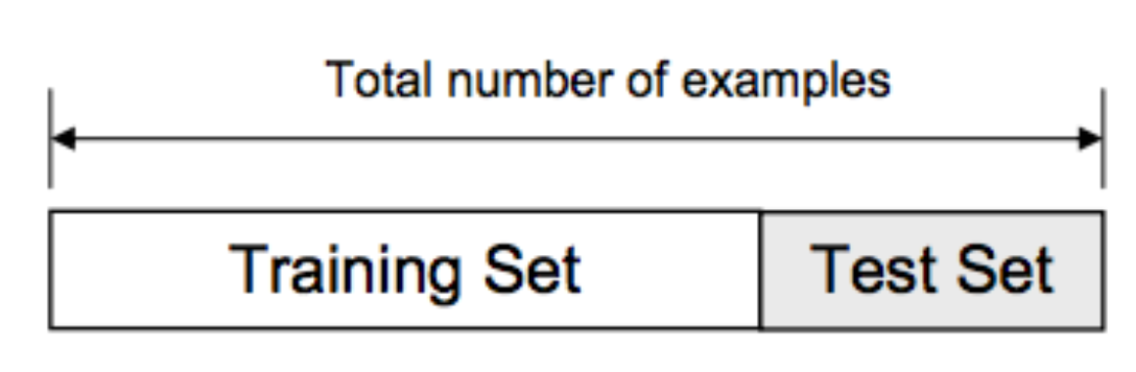
\includegraphics[width=7cm]{archivos/4.Metodologia/Datos/Separacion/DataSplit}
                        \caption{División de un conjunto de datos en datos de entrenamiento y test \cite{TrainTestSplitImage}.}
                        \label{DataSplitImage}
                     \end{figure}

            \end{enumerate}



        \subsection{Remuestreo}


            Con el objetivo de que el modelo no se vea muy afectado debido a la diferencia de las clases mayoritarias respecto a las minoritarias se hace necesaria la utilización de técnicas de remuestreo. Estas técnicas permiten operar sobre un conjunto de datos para balancearlos, y se aplican únicamente al conjunto de entrenamiento, ya que la intención  es influir sobre el aprendizaje del modelo para aumentar el rendimiento de las predicciones sobre el conjunto de test, si aplicásemos remuestreo sobre este último conjunto estaríamos falseando los resultados de las predicciones.


            En este proyecto se ha hecho uso de la generación de datos sintéticos como método de remuestreo. Estos procedimientos permiten generar datos artificiales en base a los límites que separan unas clases de otras. Más concretamente, se ha utilizado la tećnica \glsentryfull{smoteii} \cite{SMOTEII}. Este método selecciona los vecinos más cercanos de la misma clase y genera nuevas muestras en base al espacio entre la clase minoritaria y sus vecinos más cercanos.

            \glsentryshort{smoteii} ha sido utilizado para generar más muestras artificiales de los accidentes pertenecientes a las clases minoritarias (\textit{severos} y \textit{graves}). Este nuevo conjunto de datos servirá como entrenamiento para los modelos, evitando que tiendan al sobreajuste. Una vez aplicado \glsentryshort{smoteii} se obtienen 42.508 muestras de cada una de las clases de accidentes. Es útil observar cuál es la representación espacial de los datos sintéticos generados por \glsentryshort{smoteii} en deferencia a los datos originales. Para esto, se ha utilizado el método \glsentryfull{tsne} \cite{TSNEPaper}, que permite visualizar las proyecciones de datos multidimensionales en espacios bidimensionales o tridimensionales. Este modelo debe su origen a su antecesor \glsentryfull{sne}, siendo una versión optmizada de éste. Mientras que \glsentryshort{sne} proyecta los datos convirtiendo las distancias Euclídeas, entre las muestras, a probabilidades condicionales, el \glsentryshort{tsne} modifica la función de coste para proyectarlos mediante una distribución t-Student, permitiendo trabajar con gradientes simplificados. En la figura \eqref{TSNEImages} se muestran las proyecciones de \glsentryshort{tsne} (tanto la representación bidimensional como la tridimensional) sobre el conjunto de datos de entrenamiento original y aquellos que han sido generados artificialmente por \glsentryshort{smoteii}.

            El \glsentryshort{tsne} de 2D aplicado sobre los datos generados por \glsentryshort{smoteii} \eqref{TSNEImages:Train2D} nos permite observar cómo se han generado las muestras con respecto a los datos originales \eqref{TSNEImages:Clean2D} en una proyección bidimensional. Se aprecia cómo se han producido las nuevas muestras de los accidentes graves (azul) calculando la cercanía de los puntos en base a las fronteras de división.


            \begin{figure}[H]
                \centering
                \begin{subfigure}[b]{0.4\textwidth}
                    \centering
                    \includesvg[scale=0.4]{archivos/4.Metodologia/Datos/Resampling/TSNE/2d_tsne_clean}
                    \caption{T-SNE de 2 componentes aplicado a los datos originales.}
                    \label{TSNEImages:Clean2D}
                \end{subfigure}
                % Añadir el espacio deseado, si se deja la linea en blanco la siguiente subfigura ira en una nueva linea
                \begin{subfigure}[b]{0.4\textwidth}
                    \centering
                    \includesvg[scale=0.4]{archivos/4.Metodologia/Datos/Resampling/TSNE/2d_tsne_train}
                    \caption{T-SNE de 2 componentes aplicado a los datos generados por SMOTE-II.}
                    \label{TSNEImages:Train2D}

                \end{subfigure}
            \end{figure}%
            \begin{figure}[H]\ContinuedFloat
                \centering
                \begin{subfigure}[b]{0.4\textwidth}
                    \centering
                    \includesvg[scale=0.4]{archivos/4.Metodologia/Datos/Resampling/TSNE/3d_tsne_clean}
                    \caption{T-SNE de 3 componentes aplicado a los datos originales.}
                    \label{TSNEImages:Clean3D}
                \end{subfigure}
                \begin{subfigure}[b]{0.4\textwidth}
                    \centering
                    \includesvg[scale=0.4]{archivos/4.Metodologia/Datos/Resampling/TSNE/3d_tsne_train}
                    \caption{T-SNE de 3 componentes aplicado a los datos generados por SMOTE-II.}
                    \label{TSNEImages:Train3D}
                \end{subfigure}
                \caption{T-SNE de 2 y 3 componentes aplicado a los datos originales y a los generados sintéticamente (\glsentryshort{smoteii}).}
                \label{TSNEImages}
             \end{figure}



    \subsection{Algoritmo Genético}


        En este proyecto se ha hecho uso del algoritmo \glsentryshort{xgboost} para calcular los pesos asignados a cada una de las características de los accidentes. El algoritmo \glsentryshort{xgboost} tiene una serie de hiperparámetros que es necesario optimizar para obtener un buen rendimiento. Esta es una etapa crítica en el modelo presentado que requiere la utilización de un algoritmo adecuado.\\

        Para esta optimización de los hiperparámetros de \glsentryshort{xgboost}, se ha hecho uso de algoritmos evolutivos. En estos algoritmos cada individuo, perteneciente a la población de una generación, es una solución especfífica a los valores de los hiperparámetros, de tal forma que a lo largo de las iteraciones los individuos evolucionarán mediante el cruce y la mutación para dar lugar a nuevas configuraciones de hiperparámetros optimizadas \cite{GAXGBoostPaper}.

        Debido al coste computacional que tendría optimizar todos los parámetros, por la magnitud del espacio de búsqueda, se ha seleccionado un subcojunto de aquellos que más influencia tienen en el entrenamiento del modelo. En este proyecto, los hiperparámetros de cada individuo de la población son:

        \begin{enumerate}

            \item Profundidad máxima: es la máxima altura que puede tomar el árbol. Si el árbol de decisión alcanza demasiada profundidad tenderá al \textit{overfitting} ya que aprenderá relaciones complejas entre los datos que pueden deberse a ruido en los datos de entrenamiento.

            \item Peso mínimo de los hijos: es el mínimo peso que se establece a la hora de crear un nuevo nodo en el árbol. Cuando se entrena un árbol de decisión éste genera nuevos nodos en base a máxima separabilidad de los datos de entrenamiento en cada nivel. Con el límite de peso de los hijos establecemos un umbral mínimo de muestras que deben pertenecer a un nodo para realizar la separación. Un valor bajo en este parámetro permitirá crear nodos con menos muestras y por lo tanto el modelo tenderá al \textit{overfitting}.

            \item ETA: tamaño de paso utilizado para aplicar descenso por gradiente para minimizar la pérdida de los árboles anteriores.

        \end{enumerate}

        En los algoritmos evolutivos, la inicialización y mutación de los valores de los individuos viene dada por una limitación mínima y máxima. Si esta restricción no se contemplase, los hiperparámetros podrían tomar valores extremos, reduciendo así el rendimiento de entrenamiento y el de las predicciones. Por lo tanto los individuos variarán sus parámetros tomando un valor aleatorio dentro de rangos definidos. Los parámetros de las nuevas soluciones mutarán dentro de unos límites específicos para cada parámetro, establecidos como máximos y mínimos.

        \begin{table}[H]
            \small
            \centering
                \begin{tabular}{ |c|c|c| } 
                \hline
                \textbf{Hiperparámetro} & \textbf{Inicialización} & \textbf{Mutación}\\
                \hline
                    Profundidad Máxima & [1, 25] & [-6, 6]\\ 
                    Peso mínimo de los hijos & [0.01, 20.0] & [-7, 7] \\ 
                    ETA & [0.01, 1] &  [-0.3, 0.3] \\ 
                \hline

                \end{tabular}

            \caption{Límites de inicialización y mutación de los hiperparámetros de los individuos.}
            \label{InitAndMutationLimitsHyperparamsTable}
        \end{table}

        Una vez inicializados aleatoriamente los individuos de la población, se evaluarán instanciando los modelos \glsentryshort{xgboost} correspondientes. La función \textit{fitness} que evaluará cada individuo será la métrica Micro F1-score, de tal forma que en cada una de las generaciones definidas se comprobará si existe algún individuo de la población en ese momento que logre superar el Micro F1-score del mejor individuo hasta el momento.

        Una vez evaluados los individuos de una generación, los \textit{15} mejores se cruzarán para dar luegar a nuevos hijos, que tendrán una probabilidad de mutación para cada una de sus \textit{4} características. En el momento de que existan individuos repetidos en la población, estos serán eliminados para dar lugar a nuevas inicializaciones aleatorias favoreciendo así la diversidad de la población. Los parámetros del mejor individuo al cabo de las generaciones correspondientes serán los hiperparámetros del algoritmo \glsentryshort{xgboost}.


    \subsection{XGBoost}


        Una vez se han optimizados los hiperparámetros del algoritmo de clasificación \glsentryshort{xgboost}, se utiliza este para calcular los pesos de las variables utilizadas en el conjunto de datos. Este modelo entrenado tiene como entrada los datos (variables) de los accidentes de tráfico y como salida los ṕesos de estas variables \cite{XGBoostFeatureWeightsMeaning}. Estos pesos indican el grado de importancia que tiene cada característica, del conjunto de datos, a la hora de entrenar el árbol, por lo tanto, aquellas caracerísticas a las que se les asigne más peso habrán sido aquellas que han jugado un papel clave en las decisiones de los árboles. Los pesos son asignados para cada característica del conjunto de datos con el que ha sido entrenado \glsentryshort{xgboost} de tal forma que permite realizar un análisis comparativo de los atributos y saber qué predictores son más importantes.


    \subsection{Matrices}


        Las redes neuronales convolucionales (\glsentryshort{cnn}) aprenden patrones sobre la entrada de datos como matrices. Esto implica que, estas estén construidas de tal forma que se maximice la representación de la información, es decir, es necesario aplicar técnicas que posicionen cada característica en un elemento de la matriz maximizando la información de los accidentes. Por lo tanto, una vez se tienen los datos normalizados y muestreados, el siguiente paso será transferir cada una de las muestras tabulares de los accidentes a una matriz, donde a cada característica se le asignará un elemento de la matriz, de tal forma que éstas sean la entrada a las \textit{CNN}. Para este objetivo, se va a aplicar un algoritmo, que asigna las características de una muestra en representación tabular en función de la importancia que éstas presenten en una jerarquía \cite{TASPCNN}.

        Las características que provocan un accidente de tráfico pueden englobarse en una serie de elementos o categorías principales, concretamente: \textit{características del conductor, el estado de la carretera, características propias del vehículo y condiciones del ambiente} \cite{JerarquiaImagenes}. Basándonos en esto se realiza una asignación de cada característica del dataset en una de estas categorías. La tabla \eqref{JerarquiaCaracteristicasTabla} muestra las asignaciones de las variables explicativas del conjunto de datos en función de esta jerarquía.


        \begin{table}[H]
          \small
          \centering
          \begin{tabular}{ |c|c| }
               \hline
               \textbf{Categoría} & \textbf{Característica}\\

               \hline
               \multirow{4}{*}{Accidente}            & Coordenada X.\\
                                                     & Coordenada Y.\\
                                                     & Hora.\\
                                                     & Vehículos implicados.\\
                                                     & Tipo de accidente.\\

               \hline
               \multirow{2}{*}{Carretera}            & Distrito.\\
                                                     & Tipo Carretera.\\


               \hline
               \multirow{1}{*}{Ambiente}             & Estado meteorológico.\\

               \hline
               \multirow{1}{*}{Vehículo}             & Tipo de vehículo.\\

               \hline
               \multirow{4}{*}{Conductor}            & Tipo Persona.\\
                                                     & Sexo.\\
                                                     & Rango Edad.\\
                                                     & Positivo.\\

               \hline
          \end{tabular}
          \caption{Jerarquía de categorías y características.}
          \label{JerarquiaCaracteristicasTabla}
        \end{table}



        Una vez definida la jerarquía de características de los accidentes de tráfico, así como los pesos asociados a cada uno de ellos, se construyen las matrices de entrada de las redes convolucionales. Es importante remarcar que las matrices de entrada son de tamaño (\textit{5 x 5}) debido a que hay 5 categorías y, a su vez, hay como mucho 5 variables de cada categoría (ver tabla \eqref{JerarquiaCaracteristicasTabla}). Así pues, el proceso de construcción de las matrices es:

        \begin{enumerate}

            \item Generación de \textit{n} matrices inicializadas a 0, donde \textit{n} es el número de muestras en el dataset.
            \item Asignación de una fila a cada padre en función de su peso.
            \item Asignacíón de cada característica hija, en función de su peso, dentro de la fila de su padre.
        
        \end{enumerate}

        Se deben tomar las siguientes consideraciones a la hora de construir las matrices:

        \begin{enumerate}

            \item La importancia de un padre viene dada por la suma de los pesos de las características hijas.

            \item La asignación de las filas de la matriz a las características padres se realiza de forma intercalada en función de su peso. Aquel padre que más importancia tenga irá posicionado en la fila central de la matriz, el segundo padre irá posicionado por encima de éste y el tercero por debajo y así sucesivamente, de tal forma que se irá creando una estructura en la que dichos padres se interpolan entre las filas en función de su peso.

            \item Una vez se han asignado las categorías padre a las filas se realiza el mismo procedimiento con las características hijas a nivel de columna. Estas características se asignarán en una posición dentro de la fila de su categoría padre, donde aquella que más importancia tenga irá posicionada en el centro, la segunda irá posicionada a su izquierda, la tercera a la derecha y así sucesivamente.
        \end{enumerate}


        La finalidad de posicionar las características más influyentes en las zonas centrales de la matriz se debe a que las \glsentryshort{cnn} utilizan los kernels para recorrer la imagen en base a un desplazamiento, por lo tanto, estos kernels convolucionarán más veces estas posiciones donde se encuentran las caracerísticas más influyentes respecto a si se sitúan en los extremos de la matriz.

        Un ejemplo de la construcción de estas matrices se ve reflejado en la figura \eqref{FV2IExampleImage}.

        \begin{figure}[H]
            \centering
            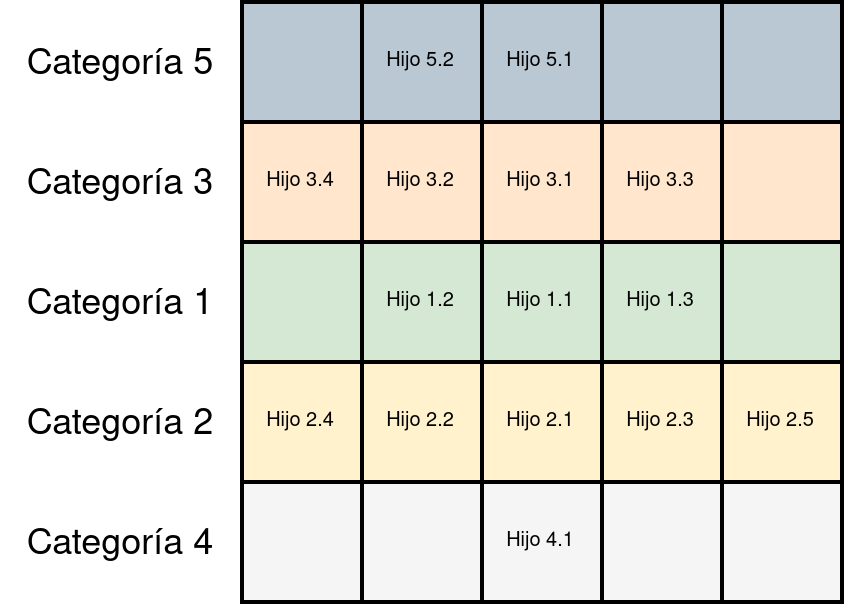
\includegraphics[width=7cm]{archivos/4.Metodologia/Matrices/FV2I}
            \caption{Ejemplo de posicionamiento de los elementos en una matriz. A las características se les asignan las filas en función de su peso y a las categorías hijas una columna dentro de la categoría correspondiente en función de su peso.}
            \label{FV2IExampleImage}
        \end{figure}

        Una vez obtenidos los índices de las matrices se posicionará cada característica de los datos en la posición asignada dentro cada matriz. Cabe recordar que estas características están normalizadas bajo \glsentryshort{zsn}, por lo que la matriz contendrá los valores de cada característica normalizados. Como resultado de este proceso se obtienen las matrices que serán la entrada de las \glsentryshort{cnn}.

    \subsection{Modelos}


        Uno de los objetivos específicos de este proyecto es la comparación del modelo de \textit{aprendizaje profundo} basado en redes neuronales convolucionales con otros modelos predictivos. Primeramente, se definen las arquitecturas que trabajan con observaciones tabulares normalizadas, es decir, aquellos que tienen como entrada un conjunto de datos de tipo real, como son \glsentryfull{gnb}, \glsentryfull{knn} y \glsentryfull{svc}. Posteriormente detallaremos las implementaciones de \glsentryshort{cnn}, que es la que trabaja con los datos en forma de matrices.

        \subsubsection{\glsentryfull{gnb}}

            El modelo \glsentryshort{gnb} asume que cada una de las variables pertenecientes al dataset son independientes. En la instanciación de este modelo no especificaremos ninguna probabilidad a priori, por lo que el modelo las calculará en función del número de muestras pertenecientes a cada clase en base al resto. En definitiva, es un algoritmo muy simple que no tiene muchos parámetros.


        \subsubsection{\glsentryfull{svc}}

            Para implementar este modelo ha sido necesario fijar el valor de regularización $C$, que representa la tolerancia a que ciertas observaciones puedan sobrepasar los márgenes del hiperplano separador. Con la finalidad de generalizar el modelo, este parámetro se ha establecido a 1. Por otro lado es necesario especificar el tipo de kernel con el que entrenará el modelo, en nuestro caso se ha utilizado un kernel radial, que medirá la distancia entre los puntos en función de la similaridad que presenten.

            Las distancias que mide el kernel radial se definen en la siguiente fórmula:

            \begin{center}
                $K(X_1, X_2) = exp (- \frac{||X_1 - X_2||^2}{2 \sigma^2})$
            \end{center}

            Donde $X_1$ y $X_2$ son los puntos que se medirán en base al kernel $K$, $||X_1 - X_2||$ es la distancia euclídea y $\sigma$ es la varianza. \glsentryshort{svc} ha sido entrenado en base a los datos de entrenamiento tabulares remuestrados por \glsentryshort{smoteii}.

        \subsubsection{\glsentryfull{knn}}

            El método \glsentryshort{knn} servirá como referencia para testar el rendimiento del resto de modelos. Al ser un método que se aplica sobre un conjunto de datos tabular original, no hará uso de las matrices generadas.

            Es necesario optimizar los parámetros de este algoritmo para conseguir un buen rendimiento, por lo que aplicaremos la técnica \textit{Grid Search} \cite{GridSearchSklearnLibrary}. Esta técnica permite la optimización de los valores de los hiperparámetros mediante una búsqueda exhaustiva en un espacio de búsqueda definido por el usuario, probando distintas combinaciones hasta cubrirlo por completo. 

            \glsentryshort{knn} construye el espacio de proyecciones mediante los datos de entrenamiento remuestreados por \glsentryshort{xgboost}, y clasifica las muestras del conjunto de test en base a la cercanía de los vecinos proyectados del conjunto de entrenamiento.


        \subsubsection{Redes Neuronales Convolucionales (\glsentryshort{cnn})}

            Una vez definidos los pasos que sigue el entrenamiento de una red neuronal y las características propias de las redes neuronales convolucionales, podemos analizar las arquitecturas de las \textit{CNNs} que se han aplicado en este proyecto. Cabe mencionar que el funcionamiento de las \textit{CNNs} únicamente difiere en el tamaño del \textit{kernel} y la forma en la que éste se desplaza debido a su dimensionalidad, por lo tanto detallaremos ambas arquitecturas de la misma forma.

            La arquitectura consta de cuatro capas convolucionales con tamaños de kernel de \textit{1 x 3} en caso de las \glsentryshort{cnn1d} y de tamaño \textit{3 x 3} para las \glsentryshort{cnn2d}. Estos kernels se proyectarán en \textit{256} canales para formar el filtro convolucional asociado a cada capa. A la salida de cada uno de los mapas de características se aplica un proceso de \glsentrylong{batchnormalization}.

            El \textit{padding} del kernel se ha establecido en 1 para ambos tipos de redes, de tal forma que las convoluciones se aplicarán añadiendo ceros en los límites de las matrices, y los \textit{strides} en (\textit{1}) para las \glsentryshort{cnn1d} y (\textit{1, 1}) para las \glsentryshort{cnn2d}, por lo tanto el desplazamiento de los kernels se hará píxel a píxel tanto en las \glsentryshort{cnn1d} como en las \glsentryshort{cnn2d}.

            A la salida de cada capa convolucional se aplica la función de activación \glsentryfull{relu}, que se comporta devolviendo el valor $0$ para aquellas entradas que sean negativas y el valor original para aquellas que sean positivas, se puede apreciar el comportamiento en la figura \eqref{RELUImage}. El rendimiento de esta función de activación en el campo de las matrices está ampliamente extendido, además, evita la probabilidad de aparición del gradiente evanescente \cite{GradientVanishingRelu}.

            \begin{center}
                $f(x) = \left\{
                               \begin{array}{lr}
                                 0 & \text{if } x<=0\\
                                 x & \text{if } x>0
                               \end{array}
                        \right.$
            \end{center}

            \begin{figure}[h]
                \centering
                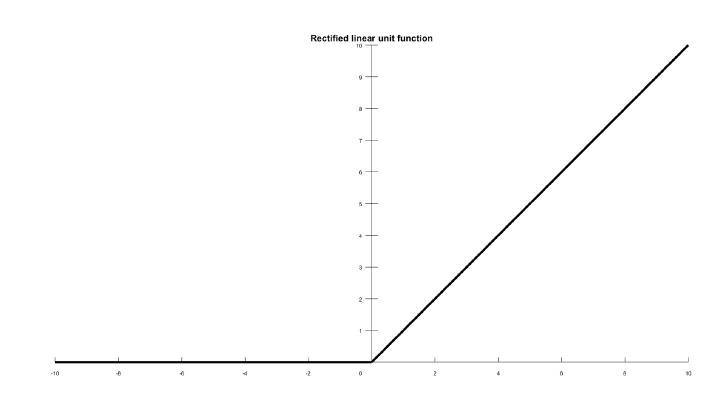
\includegraphics[width=8cm]{archivos/4.Metodologia/Modelos/CNN/RELUImage}
                \caption{Función ReLU \cite{CNNReLUImage}.}
                \label{RELUImage}
             \end{figure}

            La salida de la última capa de la convolución transforma la matriz del mapa de características de tamaño \textit{5 x 5} generada a una capa que aplanará la matriz de tal forma que la convertirá en un vector unidimensional de \textit{1 x 25}. A continuación se aplicará una capa densa que conectará cada uno de los \textit{25} nodos de la capa \textit{Flatten} con los \textit{128} nodos de la capa densa, que generará los logits antes de aplicar la última función de activación \textit{Softmax} que devolverá la clase predicha.


            Para ejemplificar la arquitectura de las \glsentryshort{cnn} propuestas se muestra el caso de la \glsentryshort{cnn2d} en la figura \eqref{TASPCNNIMAGE}


            \begin{figure}[H]
                \centering
                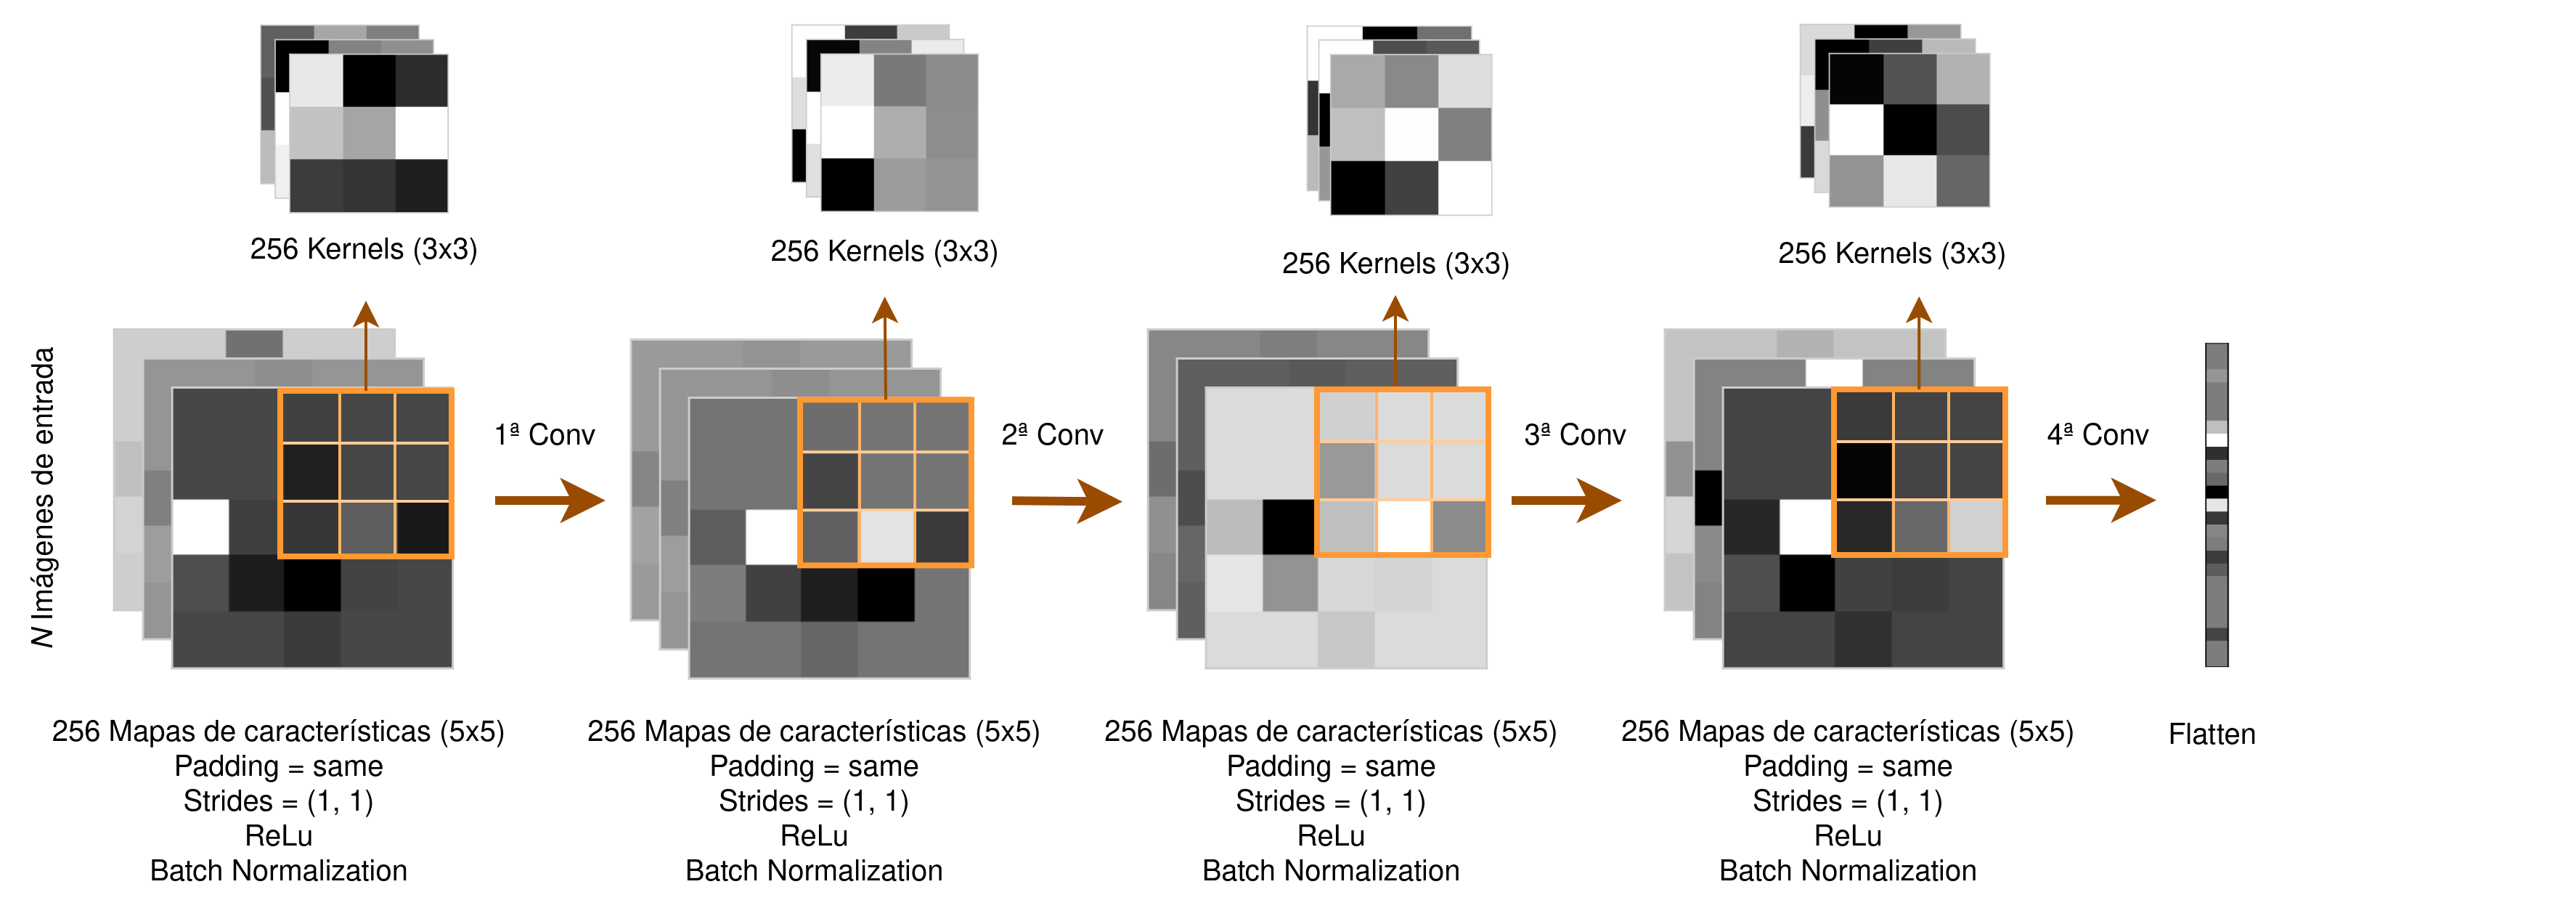
\includegraphics[width=17cm]{archivos/4.Metodologia/Modelos/CNN/2D/TASPCNN}
                \caption{Arquitectura de la CNN-2D mostrando una  kernels aprendidos durante el entrenamiento.}
                \label{TASPCNNIMAGE}
             \end{figure}


    \section{Medidas de calidad}

        A continuación se definen las métricas comúnmente utilizadas para evaluar la calidad de las clasificaciones de los modelos.


        \subsection{Métricas de clasificación}

        \begin{enumerate}

            \item Precisión: se trata el porcentaje de acierto al clasificar una clase. En el caso de este proyecto representa el porcentaje de accidentes correctos de una clase con respecto al total de accidentes predichos como dicha clase. Por ejemplo, de todos los accidentes identificados como leves, el porcentaje de los que eran leves realmente. Esta métrica se calcula dividiendo el total de verdaderos positivos respecto a la suma de verdaderos positvos y los falsos positivos.

                \begin{center}
                    Precision = $\frac{TP}{TP + FP}$
                \end{center}

            \item Exhaustividad: se trata el porcentaje de identificaciones totales del modelo para una clase. Para este proyecto la exhaustividad representa el porcentaje identificaciones correctas para una clase de accidente. Por ejemplo, del total de accidentes leves, qué porcentaje de identificaciones correctas han sido predecidas por el modelo. El cálculo de esta métrica se basa en la división de verdaderos positivos con respecto a la suma de verdaderos positivos más los falsos negativos.

                \begin{center}
                    Exhaustividad = $\frac{TP}{TP + FN}$
                \end{center}

            \item F1-Score: es una métrica que resume la precisión y exhaustividad en un solo valor para mostrar cómo de bien se realiza la clasificación de verdaderos positivos con respecto al coste de falsos negativos que esto conlleva. Es la métrica de clasificación más utilizada.

                \begin{center}
                    F1 Score = 2 $\cdot \frac{\text{Precision} \cdot \text{Exhaustividad}} {\text{Precisión} + \text{Exhaustividad}}$
                \end{center}

        \end{enumerate}

        Estas métricas se aplican para cada una de las clases a predecir, por lo que existirán tantos valores como clases se encuentren en el problema.

        \subsection{Métricas de optimización}

            Debido al desbalanceo de datos sobre el conjunto de test es necesario aplicar una función de pérdida que optimice el modelo sin tener en cuenta dicho desbalanceo. Las funciones de pérdida más comunes como la precisión total del modelo están orientadas a minimizar el error de clasificación del número total de clases. En este proyecto se usa la métrica Micro F1-score, que mide el rendimiento del modelo en función del total de clases en el conjunto de datos. En las siguientes ecuaciones se muestra cómo se calcula esta métrica en base a la micro precisión y la micro exhaustividad:

                \begin{center}
                    Micro Precision =  $\frac{ \sum_{i=1} ^ {n} TP_i} {\sum_{i = 1} ^ {n} TP_i + \sum_{i = 1} ^ {n} FP_i}$
                \end{center}

                \begin{center}
                    Micro Exhaustividad = $\frac{ \sum_{i=1} ^ {n} TP_i} {\sum_{i = 1} ^ {n} TP_i + \sum_{i = 1} ^ {n} FN_i}$
                \end{center}

                \begin{center}
                    Micro F1-score =  2 $\cdot \frac{\text{Micro Precision} \cdot \text{Micro Exhaustividad}} {\text{Micro Precisión} + \text{Micro Exhaustividad}}$
                \end{center}

        \subsection{Matrices de confusión}

        Una matriz de confusión es una técnica que permite evaluar la eficacia de un modelo respecto a la predicción de cada una de las clases objetivo. En el eje de las $X$ se muestran las etiquetas predecidas por el modelo y en el de las $Y$ las etiquetas de las clases verdaderas. De esta forma la matriz de confusión permite visualizar cómo clasifica el modelo cada una de las clases y observar a qué etiquetas asigna cada muestra sobre cualquier conjunto de datos.\\

        En la figura \eqref{MatrizConfusionExampleImage} se puede observar el esquema que sigue una matriz de confusión en base a dos posibles valores a predecir (verdadero y negativo). Las muestras clasificadas erróneamente se considerarán falsos positivos o falsos negativos en función de cómo el modelo clasifica las observaciones.

        \begin{figure}[H]
            \centering
            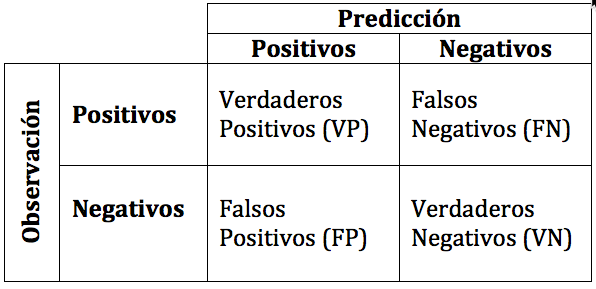
\includegraphics[width=8cm]{archivos/4.Metodologia/Metricas/MatrizConfusion}
            \caption{Ejemplo de matriz de confusión \cite{MatrizConfusionReferenciaImagen}.}
            \label{MatrizConfusionExampleImage}
         \end{figure}

